\section{Trees}
\begin{figure}
\center
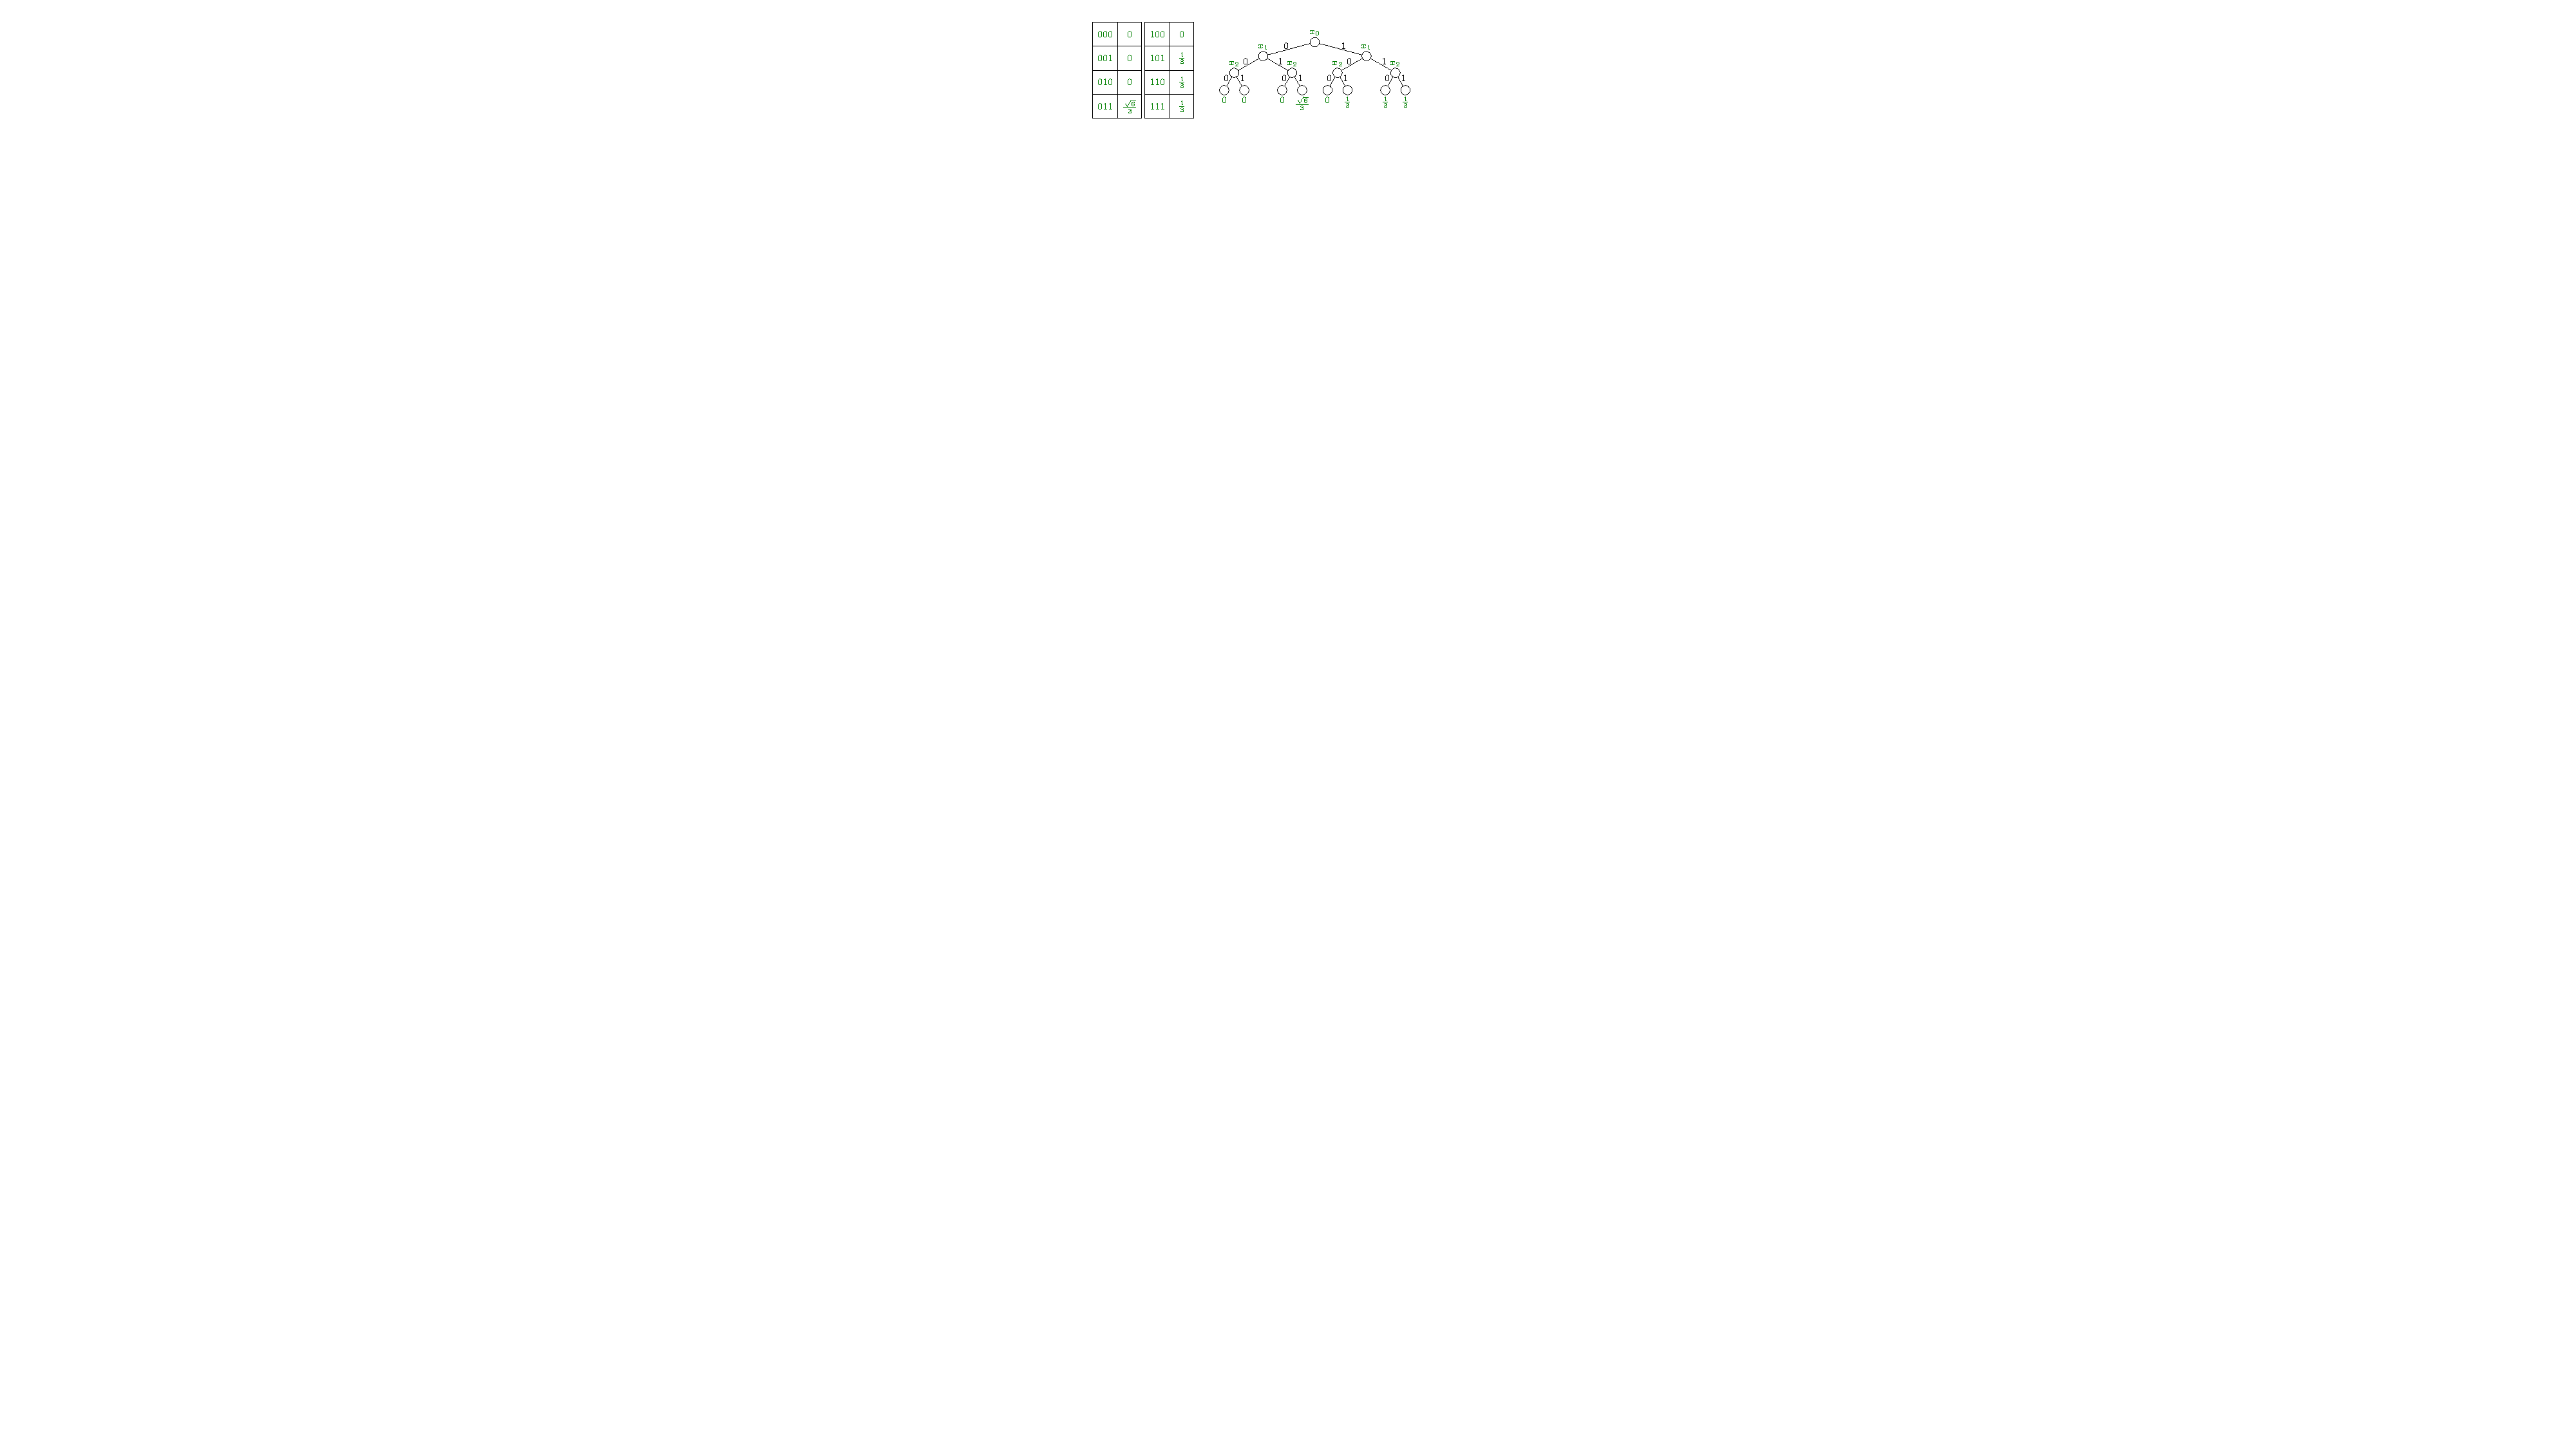
\includegraphics[]{Figures/Trees/Tree}
\caption{A quantum state with three qubits and its representation}
\label{qustate:tree:fig}
\end{figure}

A key concept in our framework is a symbolic representation of quantum states and sets of quantum states.
%
We use {\it tree automata} to instantiate the symbolic encoding.
%
Specifically, we encode a quantum state, with $\nn$ qubits as a perfect binary tree with depth $\nn$.
%
Each level of the tree corresponds to a single qubit. 
%
We might refer to the level corresponding to qubit $\xvar$ as the $\xvar$-level, and the nodes at the $\xvar$-level as the $\xvar$-nodes.
%
For an $\xvar$-node in the tree,  the left and right sub-trees corresponds to $\xvar$ being in the values $0$ and $1$ respectively.
%
Each path in the tree, from the root to a leaf, represents a computational basis state.
%
The leaves represent the complex probability amplitudes of these basis states.

Consider \cref{qustate:tree:fig}.
%
The left part shows a quantum state comprising nthree qubits.
%
On the right side, we show its tree representation.
%

\patodo{How about BDDs and classical tree automata?}


\begin{figure}
\center
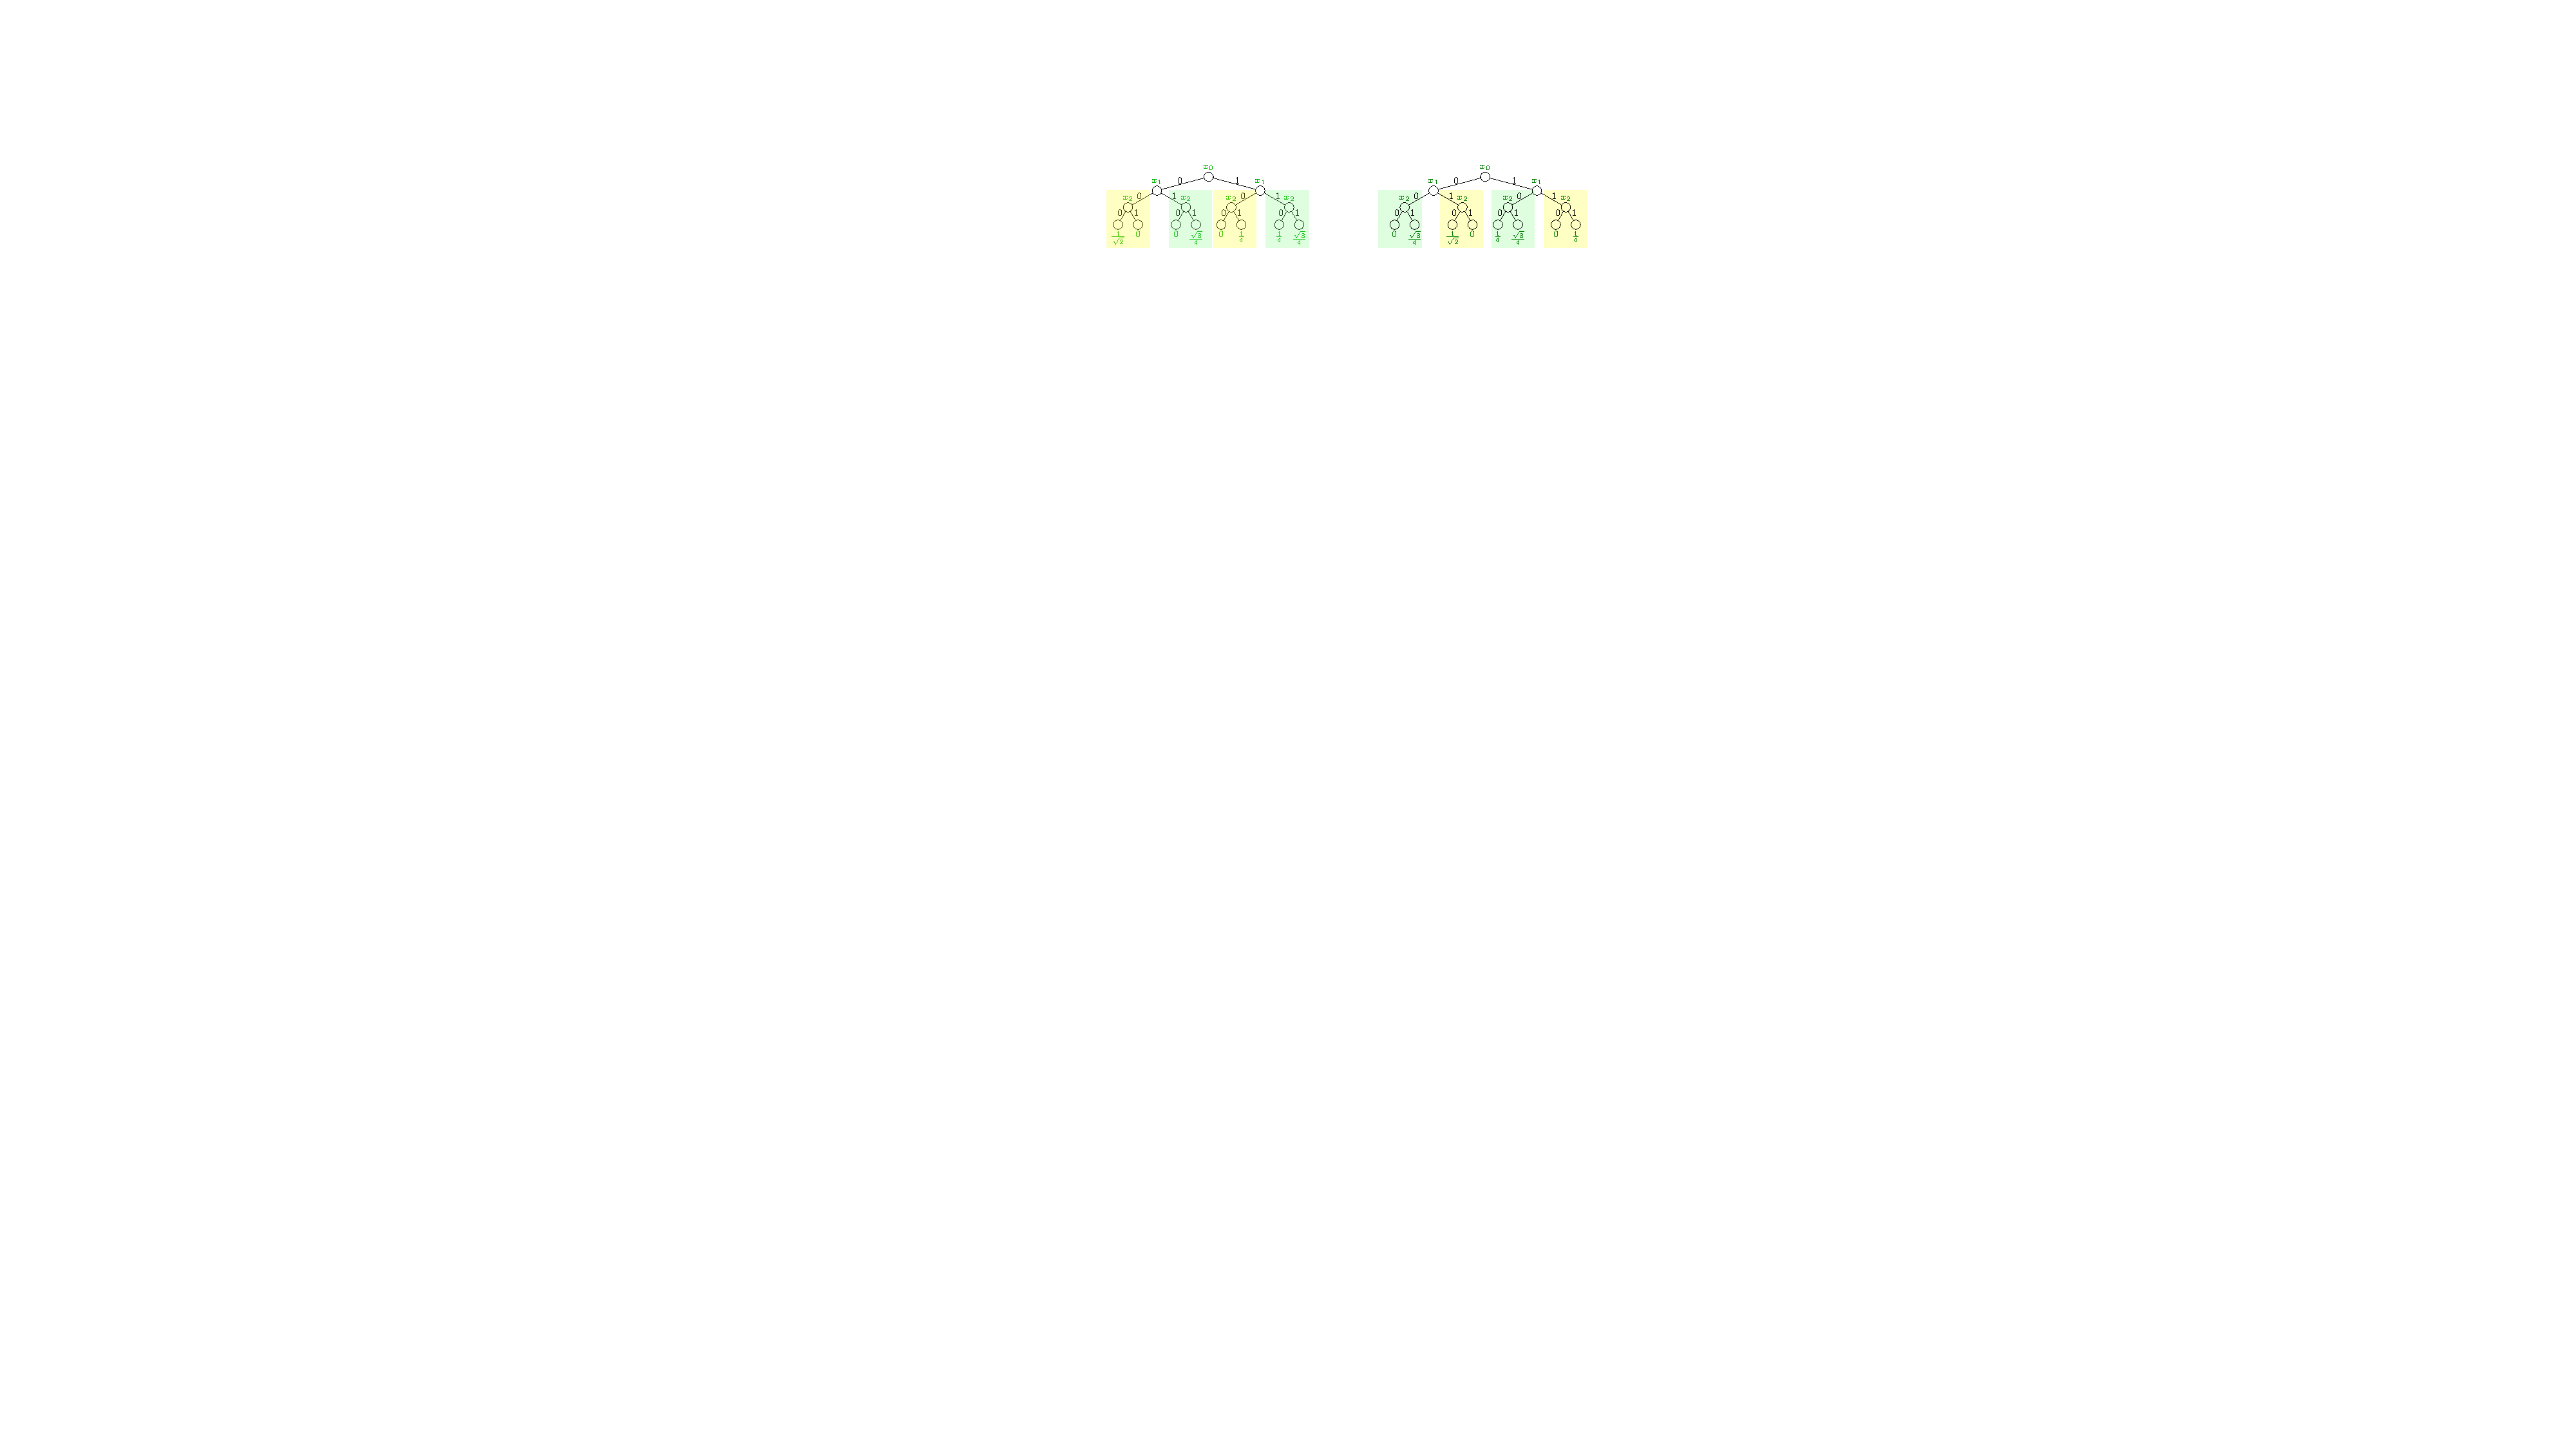
\includegraphics[]{Figures/Trees/ApplyNOT}
\caption{Applying the NOT gate to the second qubit.}
\label{apply:not:fig}
\end{figure}
%
In \ref{apply:not:fig}, we depict the result of applying the CNOT gate on the quantum state represented by the tree $\itree1$.
%
We obtain a new state represented, by the tree $\itree2$, where we swap the left- and righ-subtrres of each node at level $2$ of the tree.

\begin{figure}
\center
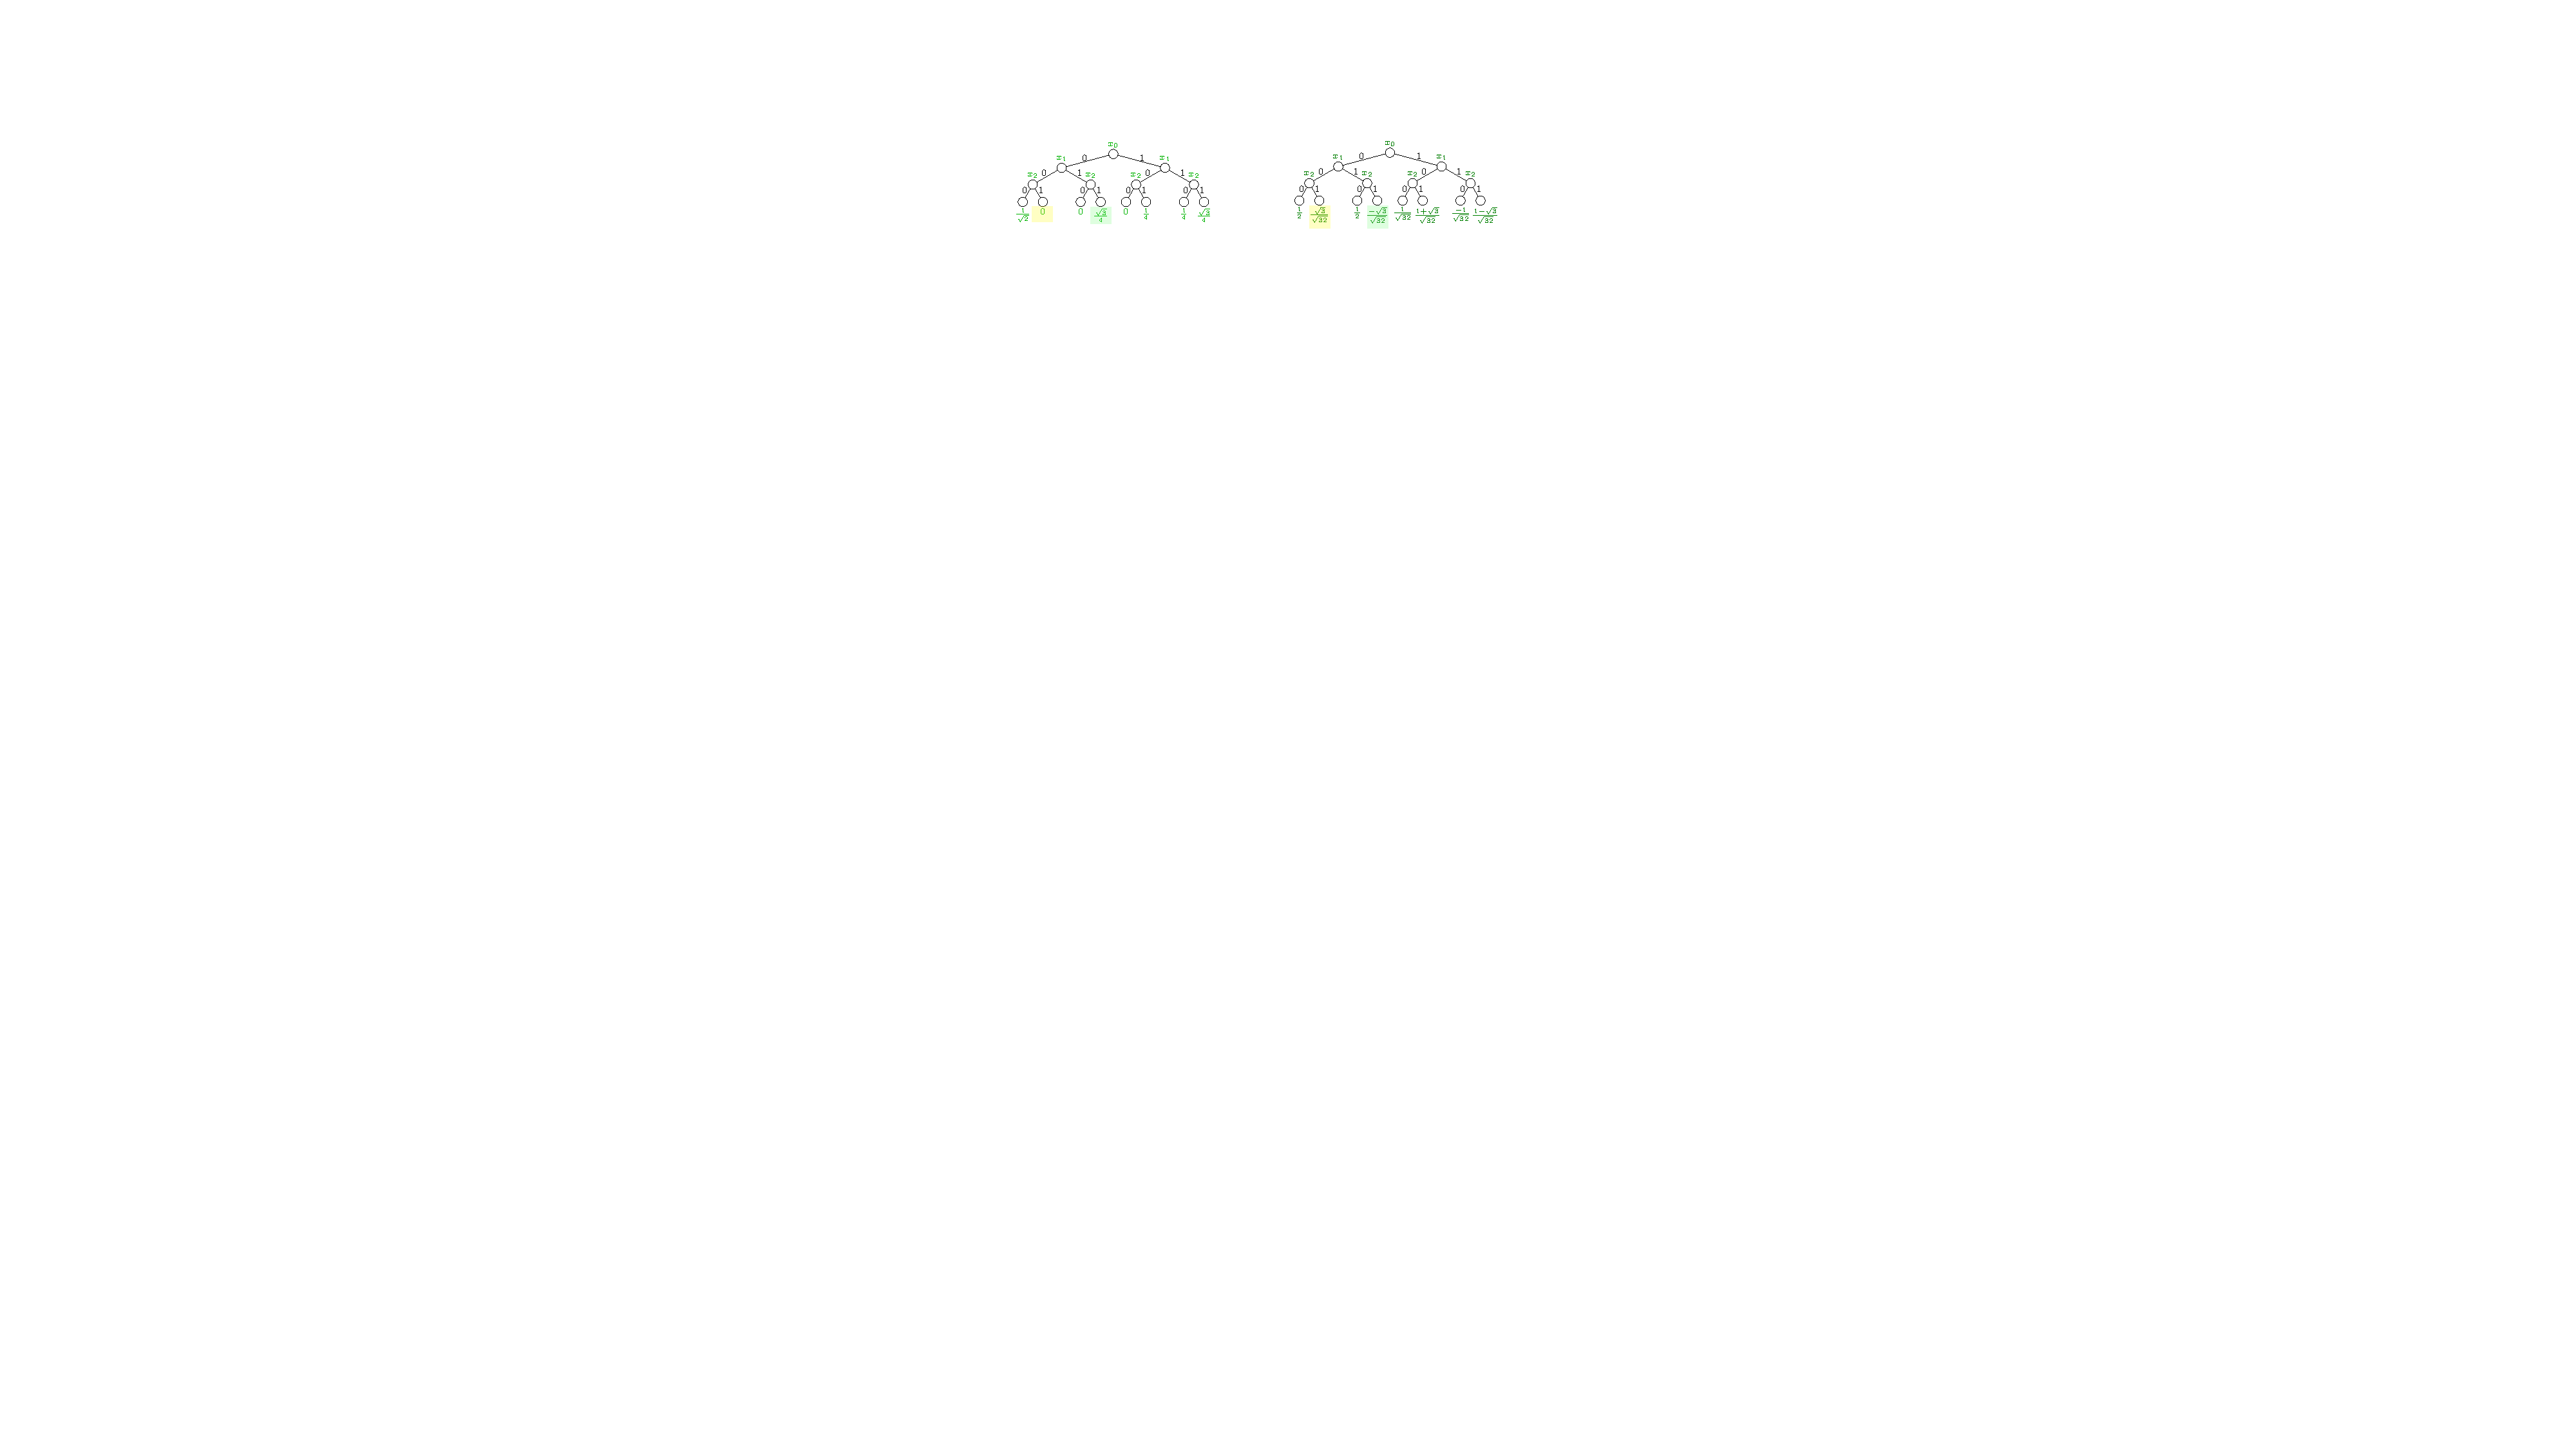
\includegraphics[]{Figures/Trees/ApplyH}
\caption{Applying the H gate to the second qubit.}
\label{apply:H:fig}
\end{figure}
